\chapter{Concepts}
\label{chp:concepts}

To set the stage for what follows, we first give a brief overview of some of the concepts in the \PDl with the help of an example shown in \fig{eg1}.

\begin{figure}[H]
  \centering
  \vspace*{-0.75em}
  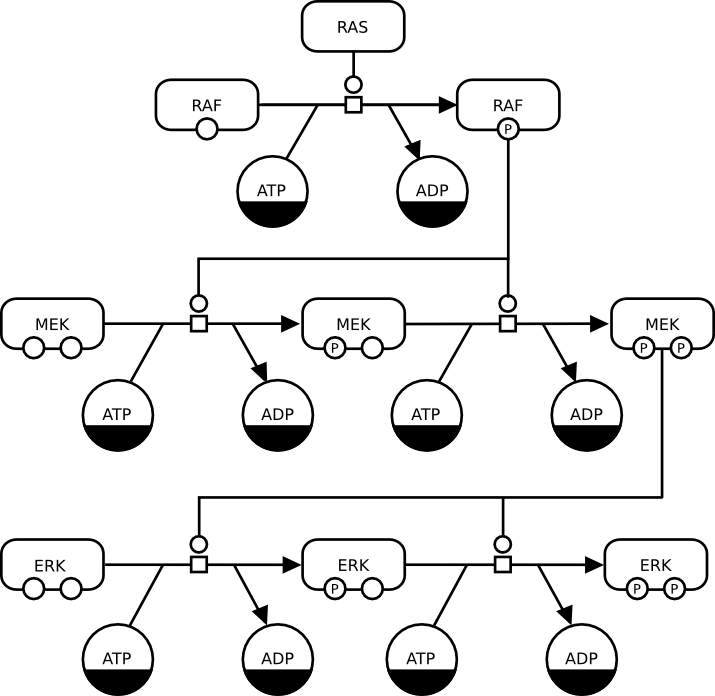
\includegraphics[scale=0.8]{examples/MAPK-only}
  \caption{This example of a \PD uses two kinds of entity pool nodes: one
    for pools of different macromolecules (\sect{macromolecule}) and
    another for pools of simple chemicals (\sect{simpleChemical}).  Most
    macromolecule nodes in this map are adorned with state
    variables (\sect{stateVariable}) representing phosphorylation states.
    This map uses one type of process node, the process node
    (\sect{process}), and three kind of connecting arc, consumption (\sect{consumption}), production (\sect{production}) and catalysis
    (\sect{catalysis}).  Finally, some entity pool nodes have dark bands
    along their bottoms; these are clone markers (\sect{cloneMarker}) indicating that the same
    pool nodes appear multiple times in the map.}
  \label{fig:eg1}
\end{figure}

The map in \fig{eg1} is a simple map for part of a mitogen-activated protein kinase (MAPK) cascade.  The larger nodes in the figure (some of which are in the shape of rounded rectangles and others in the shape of circles) represent biological materials---things like macromolecules and simple chemicals.  The biological materials are altered via processes, which are indicated in \PDl by lines with arrows and other decorations.  In this particular map, all of the processes happen to be the same: processes catalyzed by biochemical entities.  The directions of the arrows indicate the direction of the processes; for example, unphosphorylated RAF kinase processes to phosphorylated RAF kinase via a process catalyzed by RAS. Although ATP and ADP are shown as incidental to the phosphorylations on this particular graph, they are involved in the same process as the proteins getting phosphorylated. The small circles on the nodes for RAF and other entity pools represent state variables (in this case, phosphorylation sites). 

The essence of the \PDs is \emph{change}: it shows how different entities in the system process from one form to another.  The entities themselves can be many different things.  In the example of \fig{eg1}, they are either pools of macromolecules or pools of simple chemicals, but as will become clear later in this chapter, they can be other conceptual and material constructs as well.  Note also that we speak of \emph{entity pools} rather than individuals; this is because in biochemical network models, one does not focus on single molecules, but rather collections of molecules of the same kind.  The molecules in a given pool are considered indistinguishable from each other.  The way in which one type of entity is transformed into another is conveyed by a \emph{process node} and links between entity pool nodes and process nodes indicate an influence by the entities on the processes.  In the case of \fig{eg1}, those links describe consumption \sect{consumption}, production \sect{production} and catalysis \sect{catalysis}, but others are possible.  Finally, nodes in \PDs are usually not repeated; if they do need to be repeated, they are marked with \emph{clone markers}---specific modifications to the appearance of the node (\sect{cloneMarker}). The details of this and other aspects of \PD notation are explained in the following chapters.

% \tab{component-summary} summarizes the different SBGN abstractions described in this chapter.

% \newcolumntype{P}[1]{>{\raggedright\hspace{0pt}\arraybackslash}p{#1}}

% \begin{table}[bh]
%   \centering
%   \small
%   \begin{tabular}{@{}llP{2.4in}P{1.6in}@{}}
%     \toprule
%     \textbf{Component} & \textbf{Abbrev.} & \textbf{Role} & \textbf{Examples}\\
%     \midrule
%     Entity pool node
%     & EPN
%     & A population of entities that cannot be distinguished from each other
%     & Specific macromolecules or other chemical species \\[0.5em]

%     Container node	
%     & CN
%     & An encapsulation of one or more other SBGN constructs
%     & Complexes, compartments \\[1.6em]

%     Process node
%     & PN
%     & A process that transforms one or more EPNs into one or more other EPNs
%     & Process, association, dissociation \\[0.5em]

%     Arc
%     & ---
%     & Links between EPNs or CNs to PNs or CNs to indicate influences
%     & Production, catalysis, inhibition \\[0.5em]

%     Logical operators
%     & ---
%     & Combines one or several inputs into one output
%     & Boolean \emph{and}, \emph{or}, \emph{not} \\
%     \bottomrule
%   \end{tabular}
%   \caption{Summary of \PD components and their roles.}
%   \label{tab:component-summary}
% \end{table}





% \section{Entity pool nodes}\label{sec:EPNs}

% An entity pool is a population of entities that cannot be distinguished from each other, when it comes to the \SBGNPDLone map. For instance all the molecular  entities that fulfill the same role in a given process form an entity pool. As a result, an entity pool can represent different granularity levels, such as all the proteins, all the instances of a given protein, only certain forms of a given protein. To belong to a different compartment is sufficient to belong to different entity pools. Calcium ions in the endoplasmic reticulum and calcium ions in the cytosol belong to different entity pools when it comes to representing calcium release from the endoplasmic reticulum.

% The \PD contains six glyphs representing classes of material entities: \glyph{unspecified entity} (\sect{unspecifiedEntity}), \glyph{simple chemical} (\sect{simpleChemical}), \glyph{macromolecule} (\sect{macromolecule}), \glyph{nucleic acid feature} (\sect{genetic}), \glyph{multimer} (\sect{multimer}) and \glyph{complex} (\sect{complex}).  (Specific types of macromolecules, such as protein, RNA, DNA, polysaccharide, and specific simple chemicals are not defined by \PD but may be part of future levels of SBGN.)  In addition to the material entities, \PD represents three conceptual entities: \glyph{source}, \glyph{sink} (\sect{sourceSink}), and \glyph{perturbing agent} (\sect{perturbing agent}).  Material and conceptual entities can optionally carry auxiliary units such as \glyph{units of information} (\sect{unitInfo}), \glyph{state variables}  (\sect{stateVariable}) and \glyph{clone markers} (\sect{cloneMarker}).


\section{Definitions and Nomenclature}

\subsection{Language versus notation}

SBGN specifications propose symbols, ways to organise them, but also semantic rules to analyse the resulting representations. SBGN "drawings" can be translated into English, but also into computer readable formats. Those specifications really propose true languages. SBGN is therefore made up of three languages.

\subsection{What are the languages?}

\textbf{PD} is a language that permits the description of all the processes taking place in a biological system. The ensemble of all these processes constitute a Description. \textbf{ER} is a language that permits the description of all the relations involving the entities of a biological system. The ensemble of all these relations constitute a Relationship.\textbf{ AF} is a language that permits the description of the flow of activity in a biological system.

\subsection{Nomenclature}

The three languages of SBGN should be referred to as:

\begin{compactitem}
\item the Process Description language.
\item the Entity Relationship language.
\item the Activity Flow language.
\end{compactitem}

\mbox{}\\
Abbreviated as:

\begin{compactitem}
\item the PD language.
\item the ER language.
\item the AF language.
\end{compactitem}

\mbox{}\\
A specific representation of a biological system in one of the SBGN languages should be referred to as:

\begin{compactitem}
\item a Process Description map.
\item an Entity Relationship map.
\item an Activity Flow map.
\end{compactitem}

\mbox{}\\
Abbreviated as:

\begin{compactitem}
\item a PD map.
\item an ER map.
\item an AF map.
\end{compactitem}

\mbox{}\\
The corpus of all SBGN representations should be referred to as:

\begin{compactitem}
\item Process Descriptions.
\item Entity Relationships.
\item Activity Flows.
\end{compactitem}

\mbox{}\\
 The capitalization is important. PD, ER and AF are names of languages. As such they must be capitalized in English. This is not the case of the accompanying noun (language or map).

\subsection{Graph, diagram or map?}

A graph is a very technical term that belongs to mathematics and is uncommon in biology. Diagram is a concept that encompasses more than just graph. Examples are Venn diagrams for instance. Therefore, we recommend using the term map for SBGN representations. Those representations effectively permit users to travel and orient themselves in a biological system. Map is also the term most frequently used by the different communities, whether in metabolism, signaling or genomics.


